%%%%%%%%%%%%%%%%%%%%%%%%%%%%%%%%%%%%%%%%%%%%%%%%%%%%%%%%%%%%%%%%%%%%%%%%%%%%%%%%%%%%%%%
\PassOptionsToPackage{dvipsnames, svgnames}{xcolor} % paquetes para utilizar variedad de colores. ver más en http://en.wikibooks.org/wiki/LaTeX/Colors y http://www.latextemplates.com/svgnames-colors
\documentclass{beamer}  

\mode<presentation> {

% The Beamer class comes with a number of default slide themes
% which change the colors and layouts of slides. Below this is a list
% of all the themes, uncomment each in turn to see what they look like.

%\usetheme{default}
%\usetheme{AnnArbor}
%\usetheme{Antibes}
%\usetheme{Bergen}
%\usetheme{Berkeley}
%\usetheme{Berlin}
%\usetheme{Boadilla}
%\usetheme{CambridgeUS}
%\usetheme{Copenhagen}
%\usetheme{Darmstadt}
%\usetheme{Dresden}
\usetheme{Frankfurt}
%\usetheme{Goettingen}
%\usetheme{Hannover}
%\usetheme{Ilmenau}
%\usetheme{JuanLesPins}
%\usetheme{Luebeck}
	%\usetheme{Madrid}
%\usetheme{Malmoe}
%\usetheme{Marburg}
%\usetheme{Montpellier}
%\usetheme{PaloAlto}
%\usetheme{Pittsburgh}
%\usetheme{Rochester}
%\usetheme{Singapore}
%\usetheme{Szeged}
%\usetheme{Warsaw}

% As well as themes, the Beamer class has a number of color themes
% for any slide theme. Uncomment each of these in turn to see how it
% changes the colors of your current slide theme.

%\usecolortheme{albatross}
\usecolortheme{beaver}
%\usecolortheme{beetle}
%\usecolortheme{crane}
%\usecolortheme{dolphin}
%\usecolortheme{dove}
%\usecolortheme{fly}
%\usecolortheme{lily}
%\usecolortheme{orchid}
%\usecolortheme{rose}
%\usecolortheme{seagull}
%\usecolortheme{seahorse}
%\usecolortheme{whale}
%\usecolortheme{wolverine}

%\setbeamertemplate{footline}               % To remove the footer line in all slides uncomment this line
%\setbeamertemplate{footline}[page number]  % To replace the footer line in all slides with a simple slide count uncomment this line

%\setbeamertemplate{navigation symbols}{}   % To remove the navigation symbols from the bottom of all slides uncomment this line
}
\usepackage{booktabs}                       % Allows the use of \toprule, \midrule and \bottomrule in tables
\usepackage[utf8]{inputenc}                   % Para escribir tildes y eñes
\usepackage[spanish]{babel}
\usepackage{verbatim}	% Para texto plano
\usepackage{graphicx}     % Para insertar gráficas
\DeclareGraphicsExtensions{.pdf,.png,.jpg}
\usepackage{caption}
\usepackage{amsthm}
\usepackage{tikz}
\newtheorem{Teo}{Teorema}					% nuevo comando Teo, para escribir teoremas
%\usepackage{subcaption}

%%%%%%%%%%%%%%%%%%%%%%%%%%%%%%%%%%%%%%%%%%%%%%%%%%%%%%%%%%%%%%%%%%%%%%%%%%%%%%%%%%%%%%%
%---------------------------------  configuración de lisnting para código de C++
%
\usepackage{listings}	% Para códigos: C, C++, python, ver detalles en http://en.wikibooks.org/wiki/LaTeX/Source_Code_Listings
\lstset{language=C++, basicstyle=\color{DarkSlateGray}\ttfamily\footnotesize, keywordstyle=\color{RoyalBlue}\ttfamily\footnotesize, stringstyle=\color{Tomato}\ttfamily\footnotesize, commentstyle=\color{MediumSeaGreen}\ttfamily\footnotesize, morecomment=[l][\color{DarkViolet}]{\#}}

% ver variedad de colores en http://en.wikibooks.org/wiki/LaTeX/Colors y http://www.latextemplates.com/svgnames-colors
%------------------------------------------------


%----------------------------------------------------------------------------------------
%	TITLE PAGE
%----------------------------------------------------------------------------------------

\title[Formatos 3D]{{\tiny Investigación bibliográfica 1:}\\ Estructuras de datos para gr\' aficos en tres dimensiones, con \' enfasis en algoritmos de comparaci\' on.} % The short title appears at the bottom of every slide, the full title is only on the title page

\author{Jean Carlos Chavarr\' ia Hughes} % Your name
\institute[UCR] % Your institution as it will appear on the bottom of every slide, may be shorthand to save space
{
Universdad de Costa Rica \\ % Your institution for the title page
\medskip
\textit{jeancarlos.chavarria@ucr.ac.cr} % Your email address (optional)
}
\date{\today} % Date, can be changed to a custom date

\begin{document}

\begin{frame}
\titlepage % Print the title page as the first slide
\end{frame}

%\begin{frame}
%\frametitle{Overview} 	% Table of contents slide, comment this block out to remove it
%\tableofcontents 		% Throughout your presentation, if you choose to use \section{} and \subsection{} commands, these will automatically be %printed on this slide as an overview of your presentation
%\end{frame}

%----------------------------------------------------------------------------------------
%	PRESENTATION SLIDES
%----------------------------------------------------------------------------------------

%------------------------------------------------
\section{Introducction} % Sections can be created in order to organize your presentation into discrete blocks, all sections and subsections are automatically printed in the table of contents as an overview of the talk
%--------------------------------------------------------
\begin{frame}
\frametitle{Objetivos Espec\' ificos} 
%Recuerde que se realiza un capitulo de investigacion por cada objetivo especifico. Sin perder de vista el objetivo general.
\begin{enumerate}
\item Comparar las caracter\' isticas de los formatos de gr\' aficos en 3D.
\item Presentar un an\' alisis de representaciones de mallas poligonales.
%	\begin{itemize}
%	\item Mallas v\' ertice-v\' ertice.
%	\item Mallas cara-v\' ertice.
%	\item Mallas de bordes-alado.
%	\item Mallas de graficaci\' on din\' amica.
%	\end{itemize}

%\item Brindar una descripci\' on detallada de los siguientes algoritmos: 
%	\begin{itemize}
%	\item Cierre transitivo.
%	\item Algoritmo de Warshall.
%	\item Algoritmo de trayectoria m\' as corta.
%	\item 
%	\end{itemize}
%

\item Describir los tipos de visualizaci\' on cient\' ifica de conjuntos de datos:
%	\begin{itemize}
%	\item Representaci\' on de campos escalares.
%	\item Representaci\' on de campos vectoriales.
%	\item Representaci\' on de campos tensores.
%	\end{itemize}
	
\end{enumerate}
\end{frame}


%--------------------------------------------------------

\begin{frame}
\frametitle{Justificaci\' on}
Why 3D objects?
\begin{itemize}
\item Vivimos en un mundo 3D. 
\item An\' alisis cient\' ifico e industrial.
\item Implementaci\' on de algebra lineal a aplicaciones reales.
\end{itemize}
\end{frame}

\begin{frame}
\frametitle{Introducción}
\begin{itemize}
\item Relaci\' on entre figuras, imagenes, objetos 3D y estructuras de datos.
\item Visualizaci\' on cient\' ifica.
\end{itemize}

\begin{figure}[h]
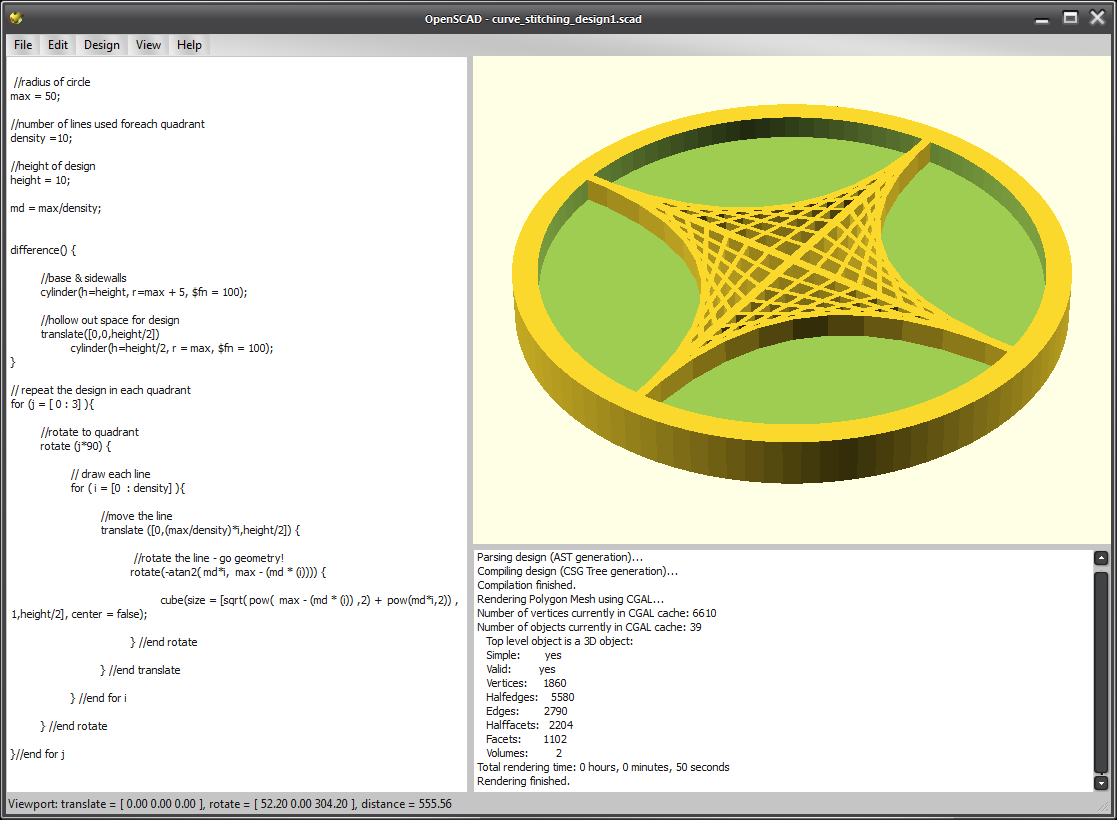
\includegraphics[width=.81\textwidth]{Images/OpenSCAD.PNG}
\centering
\end{figure}
\end{frame}

%--------------------------------------------------------
\section{Visualizaci\' on Cienti\' fica}
%--------------------------------------------------------

\begin{frame}
\frametitle{Visualizaci\' on Cient\' ifica. Qu\' e es y para que sirve}
El mapeo de representaciones hechas por la computadora a representaciones precept\' uales, con t\' ecnicas de codificaci\' on para maximixar el entendimiento  con los seres humanos.

\begin{block}{Campos Escalares}
Se refiere a conjuntos de datos que se pueden distribuir en el tiempo o en posiciones del espacio. Temperatura, presi\' on, resistencia, reflectividad, densidad.
\end{block}

\end{frame}
\begin{frame}



\begin{block}{Campos Vectoriales }
Posee 3 valores escalares, uno para cada posici\' on del espacio y una forma de representarlos es por medio de flechas que indiquen la magnitud y direcci\' on. 
\end{block}
\begin{figure}
\begin{tikzpicture}
\def \angle{pi/8}
\pgfmathsetmacro{\dang}{deg(\angle)}
\draw (0, 0) grid (4, 3);

\foreach \x/\k in {0.5/1, 1.5/2, 2.5/3, 3.5/4} {
  \foreach \y in {0.5, 1.5, 2.5} {
      \fill (\x,\y) circle[radius=1pt];
     %  \draw[->,thick]  (\x, \y) -- ++(\k*\dang:1);
	 \draw [thick] (\x,\y) --++(\k*\dang:1);
    }
}

\end{tikzpicture}
\end{figure}

\end{frame}

\begin{frame}


\begin{block}{Campos Tensoriales}
Posee 9 componentes y se representa con una matriz 3x3. Ejemplos puedes ser el tensor de presi\' on de materiales anisotr\' opicos.
\end{block}
%\end{frame}

%----------------------------------------------


%\begin{frame}
\frametitle{Qu\' e es y para que sirve}
\begin{figure}[h]
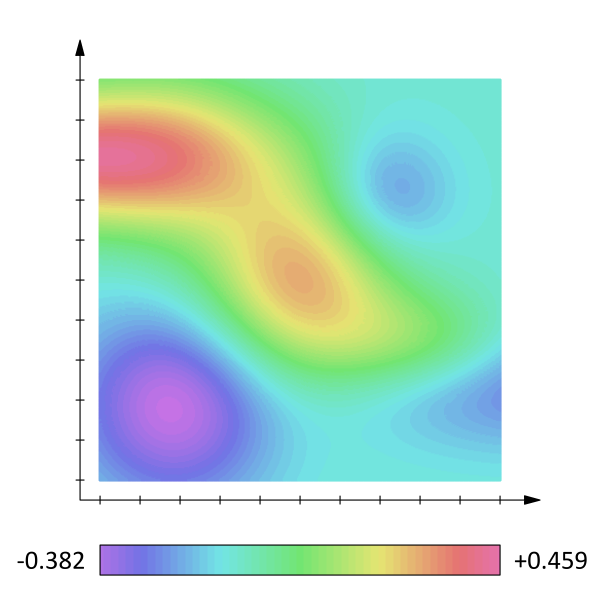
\includegraphics[width=.81\textwidth]{Images/Scalar_field.png}
\centering
\end{figure}

\end{frame}


%--------------------------------------------------------
\section{Formatos 3D}
%--------------------------------------------------------

\begin{frame}
\frametitle{Formatos: BVH}
\begin{itemize}
\item Desarrollado por BioVision y enfocado en movimientos humanos.
\item Dos partes principales, el encabezado \textbf{HIERARCHY} y el \textbf{MOTION}.
\item La primera define los segmentos: \textbf{OFFSET, CHANNELS y JOINT}.
\item La segunda define el n\' umero de \textit{frames}, el \textit{frame time}, y la informaci\' on capturada de movimiento.
\end{itemize}
\begin{figure}[hbtp]
%\caption{Uso en la biomedicina}
\centering

\includegraphics[scale=0.25]{Images/bvh1.png}
\end{figure}
\end{frame}
%---------------------------------------------
\begin{frame}
\begin{figure}[hbtp]
%\caption{Uso en la biomedicina}
\centering
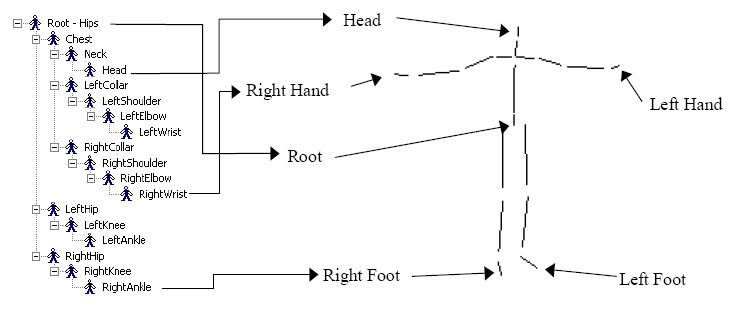
\includegraphics[scale=0.65]{Images/bvh2.jpg}
\end{figure}
\end{frame}

\begin{frame}
\frametitle{Formatos: C3D}
\begin{itemize}

\item Doctor Andrew Dainis en 1987, consigui\' on aceptaci\' on en  laboratorios de biomedicina en Bethesda, Maryland.

\item Preserva informaci\' on que describe el tipo de dise\~ no f\' isico utilizado del laboratorio, tal como posiciones de platos, conjunto de marcas y tipos de canales empleados y EMG.

\item Alamacena informaci\' on del paciente como nombre, edad, peso, longitud de piernas, etc.

\begin{figure}[hbtp]
%\caption{Uso en la biomedicina}
\centering
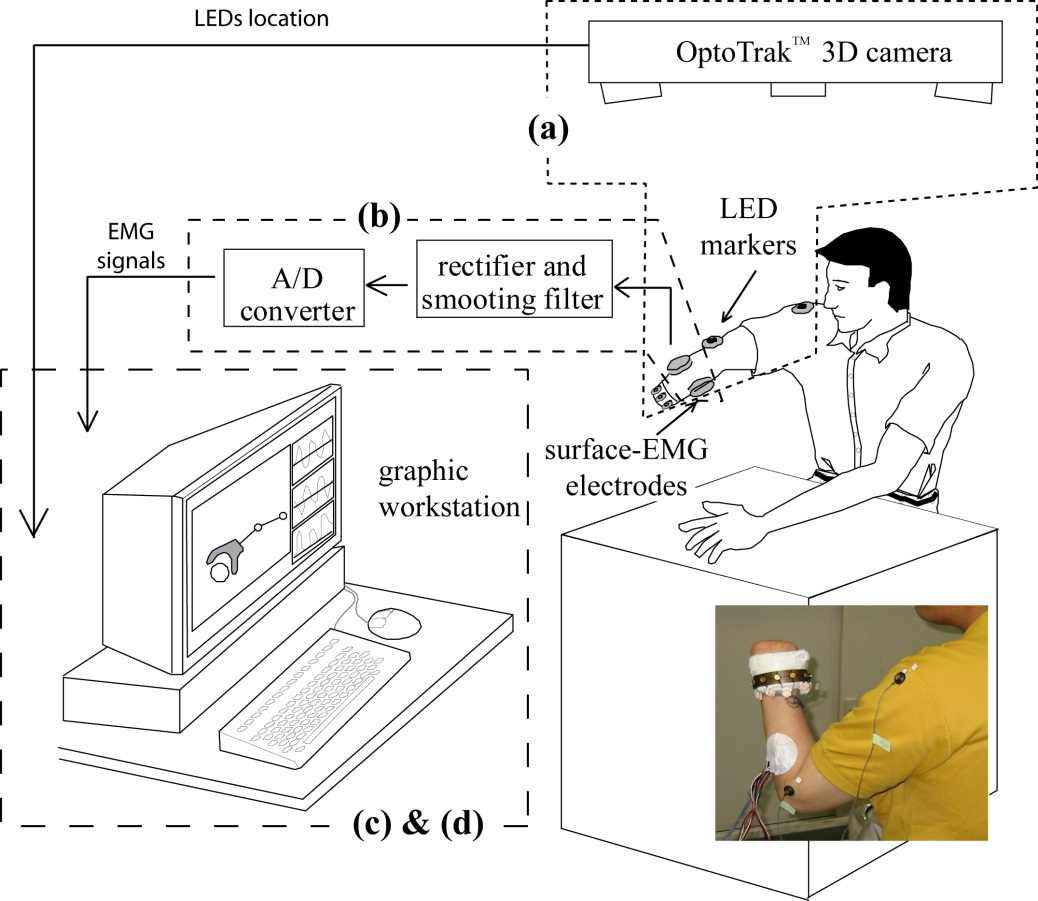
\includegraphics[scale=0.45]{Images/image22.jpeg}
\label{firg:c3d1}
\end{figure}

\end{itemize}
\end{frame}
%---------------------------------------------
\begin{frame}
\frametitle{Formatos: FBX}
\begin{itemize}
\item Desarrollado por Kaydara. Ahora due\~ no Autodesk desde 2006.
\item Similar al BVH en tanto que tiene dos secciones importantes: el ROOT y los Hijos.
\item Dirigido a las aplicaciones de simulaci\' on de objetos y animaci\' on en 3D, debido a que trabaja con muchas propiedades que sirven para caracterizar los objetos f\' isicos.
\item Datos: L\' imites de transformaciones, espacios y herencia, luz, c\' amara, null data, mesh data, armadura, textura, etc.
\begin{figure}[hbtp]
%\caption{Uso en la biomedicina}
\centering
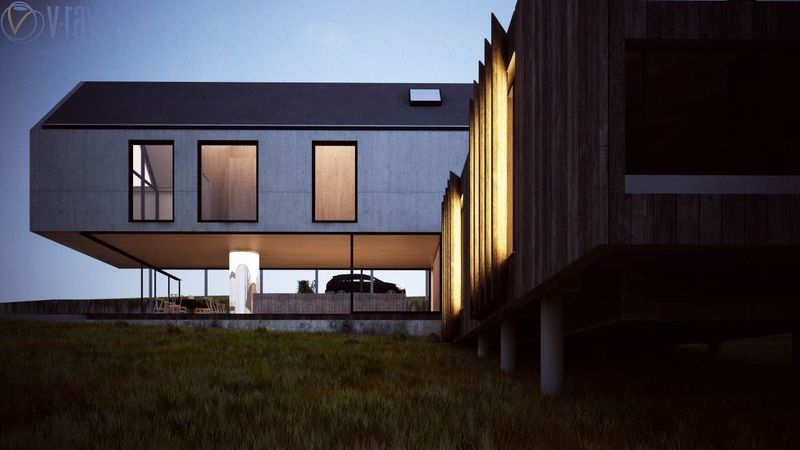
\includegraphics[scale=0.45]{Images/fbx1.jpg}
\label{firg:c3d1}
\end{figure}
\end{itemize}
\end{frame}
%---------------------------------------------
\begin{frame}
\frametitle{Formatos: POV}
\begin{itemize}
\item Vigente desde el a\~ no 1993.
\item Utiliza la t\' ecnica llamada \textbf{Ray Tracing}.
\item Permite la descripci\' on de escenas  de manera matem\' atica y utiliza efectos como la reflexi\' on, transparencia y luminosidad. Adem\' as, tiene la capacidad de crear imagenes muy realistas utilizando esta t\' ecnica y generar imagenes tipo TGA o GIF.
\item La informaci\' on almacenada en un POV es un conjunto de descriptores de escenas: c\' amaras, objetos y fuentes de luces. 
\end{itemize}
\end{frame}
%---------------------------------------------
\begin{frame}
\frametitle{Ray Tracing}
\begin{figure}[h]
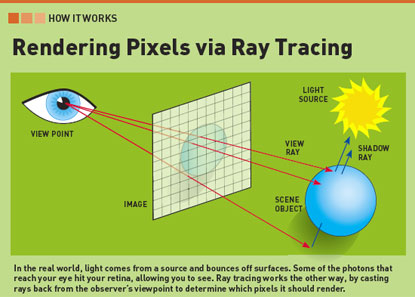
\includegraphics[width=.70\textwidth]{Images/renderingpixels.jpg}
\centering
\end{figure}
\end{frame}
%---------------------------------------------


%\begin{frame}
%\frametitle{Formatos: SKP}

%\end{frame}

%--------------------------------------------------------
\section{Representaci\' on en pol\' igonos}
%--------------------------------------------------------
\begin{frame}
\frametitle{Polygon Mesh: Elementos}
\begin{block}{Caras}
Se refiere a un conjunto cercano de bordes que conforman un pol\' igono establecido, generalmente un tri\' angulo pero tambien puede ser un cuadril\' atero u otro.
\end{block}
\begin{block}{V\' ertices}
Contiene coordenadas en 3D de cada uno de los v\' ertices que conforman los pol\' igonos limitadores de la superficie.  Puede conterner informaci\' on como color, vector normal y textura.
\end{block}
\begin{block}{Bordes}
Contiene definiciones de la conexi\' on de cada borde en t\' erminos de \' indices de nodos y especif\' ica las conexiones de v\' ertices.
\end{block}

\end{frame}

\begin{frame}
\begin{figure}[hbtp]
%\caption{•}
\centering
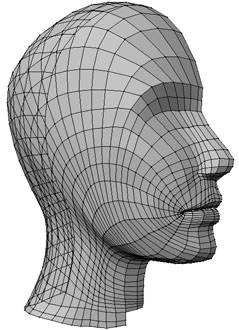
\includegraphics[scale=0.5]{Images/polygon1.jpeg}
\end{figure}
\begin{figure}[hbtp]
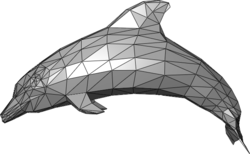
\includegraphics[scale=0.5]{Images/polygon2.png} 
\end{figure}
\end{frame}


%---------------------------------------------
\begin{frame}
\frametitle{Polygon Mesh: Representaciones}
\begin{block}{Cara V\' ertice}
Representa un conjunto de caras y v\' ertices y t\' ipicamente es aceptado por los hardwards de procesamiento gr\' afico actual debido a su gran presici\' on y redimiento.
\end{block}
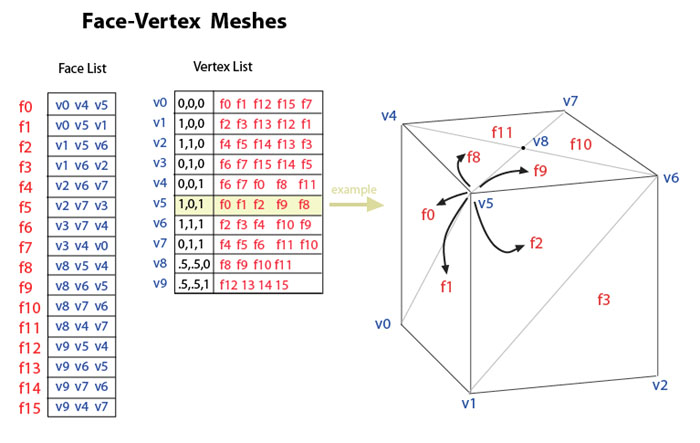
\includegraphics[scale=0.49]{Images/Mesh_fv.jpg} 
\end{frame}
%---------------------------------------------
\begin{frame}
\frametitle{Polygon Mesh: Representaciones}
\begin{block}{V\' ertice V\' ertice}
Represeta a objetos conjuntos de v\' ertices conectados con v\' ertices y es la manera m\' as simple y ligera, pero no la m\' as precisa.
\end{block}
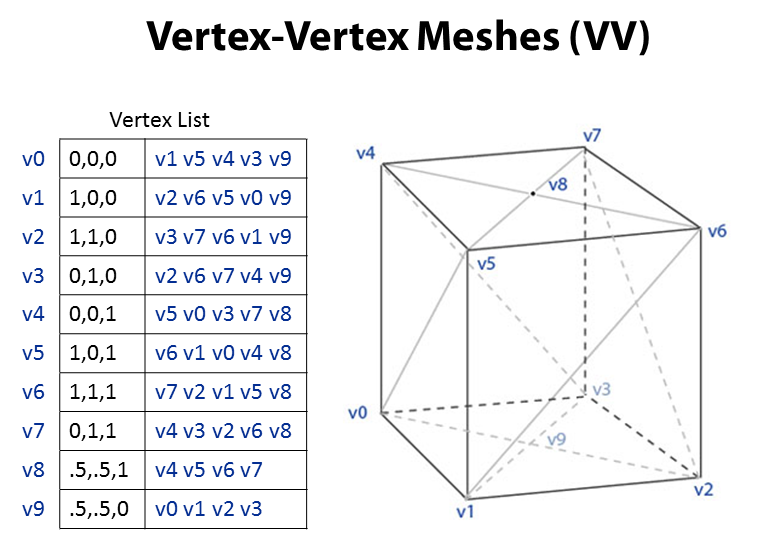
\includegraphics[scale=0.50]{Images/Vertex-Vertex_Meshes_(VV).png} 
\end{frame}
%---------------------------------------------
\begin{frame}
\frametitle{Polygon Mesh: Representaciones}
\begin{block}{Eje alado}
Baumgart en 1975. Provee informaci\' on sobre los tres elementos fundamentales: caras, bordes y v\' ertices.
\end{block}
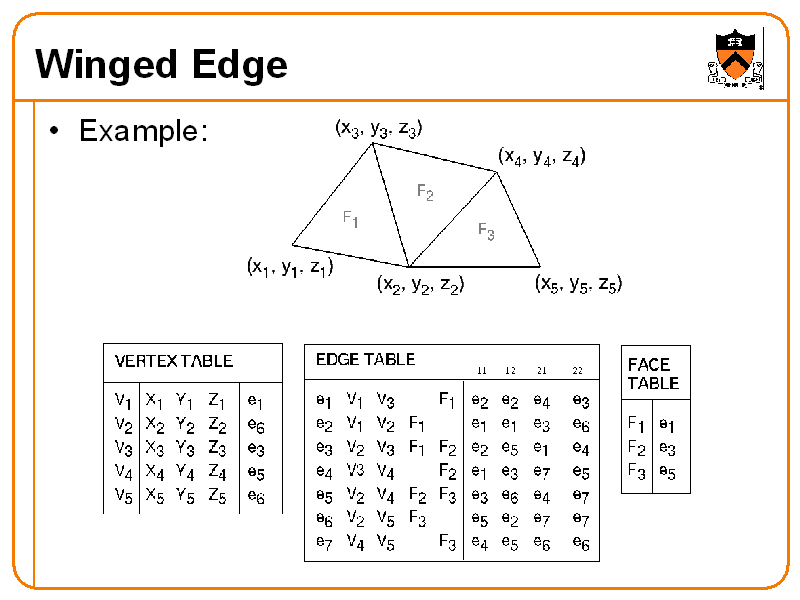
\includegraphics[scale=0.27]{Images/img028.png} 
\end{frame}
%---------------------------------------------

%%%%%%%%FINAL%%%%%%%%%%%%%%%%%








%-----------------------------------------------


%----------------------------------------------------------------------------------------
\begin{frame}
\frametitle{Referencias}
\begin{itemize}
\item Foundations of Computer Graphics: Berkeley.
\item Geometric Modeling for Computer Graphics: Princeton.
\item Computer Graphics: MIT.
\item Solid Modeling: Berkeley.
\end{itemize}
\begin{center}
{\Huge Thanks!}
\end{center}
\end{frame}

\end{document} 
